\chapter{¿Será estable un gran sistema complejo?}
\setlength{\parindent}{0cm}
Dentro del marco de los sistemas complejos se manejan varias ramas muy interesantes que le dan su esencia, desde los sistemas dinámicos discretos, dinámica no lineal, teoría de redes complejas, termodinámica fuera de equilibrio, modelos basados en agentes, entre otras. Cada una de ellas aporta un valioso contenido al sistema complejo que se quiera estudiar y analizar dependiendo de sus componentes. Delimitar el área de los sistemas complejos aún resulta una labor complicada debido a su gran \textit{diversidad}, sin embargo, se sabe de la existencia de ciertas características que todo sistema complejo comparte. Los sistemas complejos cuentan con entes: \textit{conectados, interdependientes, dependientes del camino, emergentes} entre otros. El presente trabajo tiene como propósito mostrar al lector cada una de estas características a través del sistema que se va a proponer como piedra angular.\\
\\
Antes que nada, será necesario delimitar las áreas que intervendrán en la discusión constante de este texto. Se ocupará un \textit{sistema dinámico no-lineal} bajo el soporte de una \textit{red compleja}. Como se ha mencionado anteriormente la dinámica no lineal es la rama de los sistemas dinámicos continuos en donde el comportamiento del sistema no se rige por la suma de los comportamientos de sus descriptores, sino que el ensamble mismo genera un comportamiento que va más allá de ello. Por otro lado las redes complejas es la extensión de la \textit{teoría de grafos} aplicada a escenarios comunes de la naturaleza y de la vida cotidiana, tales como redes ecológicas, redes sociales, redes comerciales etc. Su importancia radica en las propiedades que se le pueden extraer para interpretar información sobre la estructura de la red.
\newpage
\section{Antecedentes}\label{sec:Antecedentes}

Por primera vez en 1978, Robert May realizó un trabajo trascendente para los sistemas complejos en el ámbito de la estabilidad \cite{may1972will}, si se considera una red ecológica en la que participan $N\gg 1$ especies, la pregunta central es ¿de qué dependerá de que dicho sistema pueda ser estable o no? esta pregunta pretende indagar las condiciones de la red ecológica que hacen que el sistema sea estable; en términos matemáticos se refiere a que exista una tendencia hacia un atractor global, donde convergen todas las soluciones. En otras palabras, cómo deben ser los parámetros que gobiernan al sistema y que hacen que las poblaciones que lo constituyen se estabilicen al cabo de cierto tiempo y que además sean resistentes ante perturbaciones externas. Para definir estas redes ecológicas, May define un sistema no lineal de carácter
$$\frac{dX(t)}{dt}=\textbf{F}(X(t))$$
Donde $\textbf{F}:\mathbb{R}^n\to\mathbb{R}^n$ son las ecuaciones no lineales que constituyen la dinámica de cada población del sistema y $X(t)=(x_1(t),...,x_n(t))$ son las poblaciones en sí. Usando teoría de perturbaciones \cite{may2019stability}, se quiere explorar que sucede alrededor de un punto crítico: $\textbf{F}(X^*(t))=\vec{0}$ y para ello se tiene la ecuación
$$X(t)=X ^*+\textbf{p}(t)$$
donde $\textbf{p}(t)$ es en concreto el conjunto de perturbaciones alrededor de $X^*$. Realizando una expansión en series de Taylor se tiene 
$$\frac{d}{dt}\left (X^*(t)+\textbf{p}(t)\right )=\textbf{F}(X^*)+\left .\frac{d\textbf{F}}{dX}\right  |_{X^*}\textbf{p}(t)+\mathcal{O}(\textbf{p}^2)$$
Considerando que $\textbf{p}(t)$ son pequeñas perturbaciones, se pueden despreciar los términos no lineales y quedarnos únicamente con la primera derivada. Al reducir la ecuación anterior, finalmente se tiene 
$$\frac{d\textbf{p}(t)}{dt}=A\textbf{p}(t)$$
donde $A$ es una matriz cuadrada a la que May denomina como \textit{community matrix}\footnote{También conocida como matriz de interacciones. Es considerada una red ecológica en donde cada renglón corresponde con una especie y las columnas representa su respectiva interacción con otras especies.} y sus elementos son tal que $a_{ij}=\left .\frac{\partial f_i(X)}{\partial X_j}\right |_{X^*}$ con $f_i\in\textbf{F}$. Esta es una forma de ver al sistema de manera local alrededor del punto de crítico, realizar esta aproximación es definir un plano tangente en $X^*$ y así tener la capacidad de poder investigar que sucede aquí, en términos de la dinámica y estabilidad. El gran beneficio de este ejercicio es que permite explorar el sistema, que es no lineal, de forma local alrededor de un punto crítico con base en un sistema que si es lineal y que es más fácil de manipular. Al resolver este sistema lineal con la matriz $A$, se determinan sus valores propios y la siguiente solución
$$\textbf{p}(t)=\sum_{j=1}^N c_{j}e^{\lambda_{j}t}\vec{v}_j$$
Donde los $\lambda_{j}$ son el conjunto de valores propios de $A$ y los $\vec{v}_j$ sus vectores propios asociados. De esta ecuación se puede percibir que el signo de los valores propios es sustancial para que el sistema sea estable o no. Si todos ellos tienen parte real negativa, entonces será estable de lo contrario (con al menos uno que no lo sea) será inestable para $t\to\infty$. Es por esta razón que es sumamente importante la matriz del sistema linealizado, pues no será necesario determinar cada vector propio asociado para ver el tipo de estabilidad de $X^*$, únicamente basta con evaluar el signo de los valores propios y concluir. Por esta razón May ha decidido concentrarse en estas matrices de interacción para analizar sus cualidades y propiedades, dejando de lado todo ese procedimiento para llegar a ellas.
\\
\\
May propone una forma de definir estas matrices de interacción. Primeramente establece que los valores de la diagonal de $A$ tienen que estar fijados a un número real $-d$ ya que considera que estos valores fungen el papel de auto-regulación de cada una de las especies; si el sistema resulta estable o no, es importante que considere esta característica. Posteriormente, el resto de las entradas de la matriz $a_{ij}\in A$ con $i\neq j$ están sampleadas a partir de una distribución normal, centrada en $\mu=0$ y con desviación estándar $\sigma$. La regla para samplear cada entrada de la matriz se va a dar con base en un parámetro $C $ al que denomina \textit{conectancia}, en donde cada entrada de la matriz con $i\neq j$ tiene una probabilidad $C$ de conectarse y por lo tanto $a_{ij}=x\in\mathcal{N}(0,\sigma)$, y consecuentemente $1-C$ de no hacerlo $ a_{ij}=0$.\\
\\
%%CHECKPOINT 31marzo2025
Al parámetro $\sigma$ también se le conoce como fuerza de interacción promedio, y los valores de la distribución son los pesos de los enlaces entre especies. Estos parámetros, en conjunto con el número de entes interactuantes $N$: define la complejidad del sistema en términos de la estabilidad; habrá condiciones de $C$ y de $\sigma$ para los que el sistema sea estable y otras donde no lo será. Estas condiciones están bien estudiadas y definidas, y las conclusiones se pueden consultar en \cite{may1972will}. En próximos capítulos se mencionarán estas condiciones con cierta precisión. 
\\
\\
Un primer resultado que presenta es para cuando uno de estos sistemas es estable, se visualiza que la distribución de valores propios en el plano complejo se ajusta adecuadamente a un círculo con centro y radio $-d$, tal y como esta definida la diagonal de la matriz de interacciones $A$. A este hallazgo se le conoce como \textit{Ley Circular}, y en el caso de que el sistema no fuera estable entonces los valores propios se salen de este confinamiento, visualizando algunos de ellos con parte real positiva.
\newpage
Ya que la estabilidad de los sistemas dados por las matrices de interacción de May dependen exclusivamente de los parámetros que las construyen ($\sigma$, $C$ y $N$), existe un parámetro acoplado que define el umbral de estabilidad \cite{may1972will} el cual es  
\begin{equation}\label{eqn:paramMay}
	\sigma<(NC)^{-1/2}
\end{equation}
del que se puede obtener $\sigma\sqrt{NC}<1$, considerando el caso $d=1$. Si se fijara la $N$ y se variaran los otros dos parámetros, podrían haber diversos escenarios de estabilidad en concreto uno que de dependa de la $C$ (fijando $\sigma$) y otro que dependa de $\sigma$ (fijando $C$). \ Sin embargo se irá viendo más adelante que entre más grande sea el sistema ($N\gg1$) es menos probable que existan escenarios estables, pues al ir aumentando el número de interacciones posibles, hace al sistema más complejo de describir. Para hallar escenarios $\sigma$ favorables a sistemas estables con $N\gg 1$, se debe ajustar por lo menos $C\propto\frac{1}{N}$ lo que sugiere que $C$ será muy chica. Para hallar el caso $C$ favorable, se ajusta la desigualdad así: $C<(N\sigma^2)^{-1}$ y por consiguiente $\sigma\propto\frac{1}{\sqrt{N}}$.
\begin{figure}[h!]
	\centering
	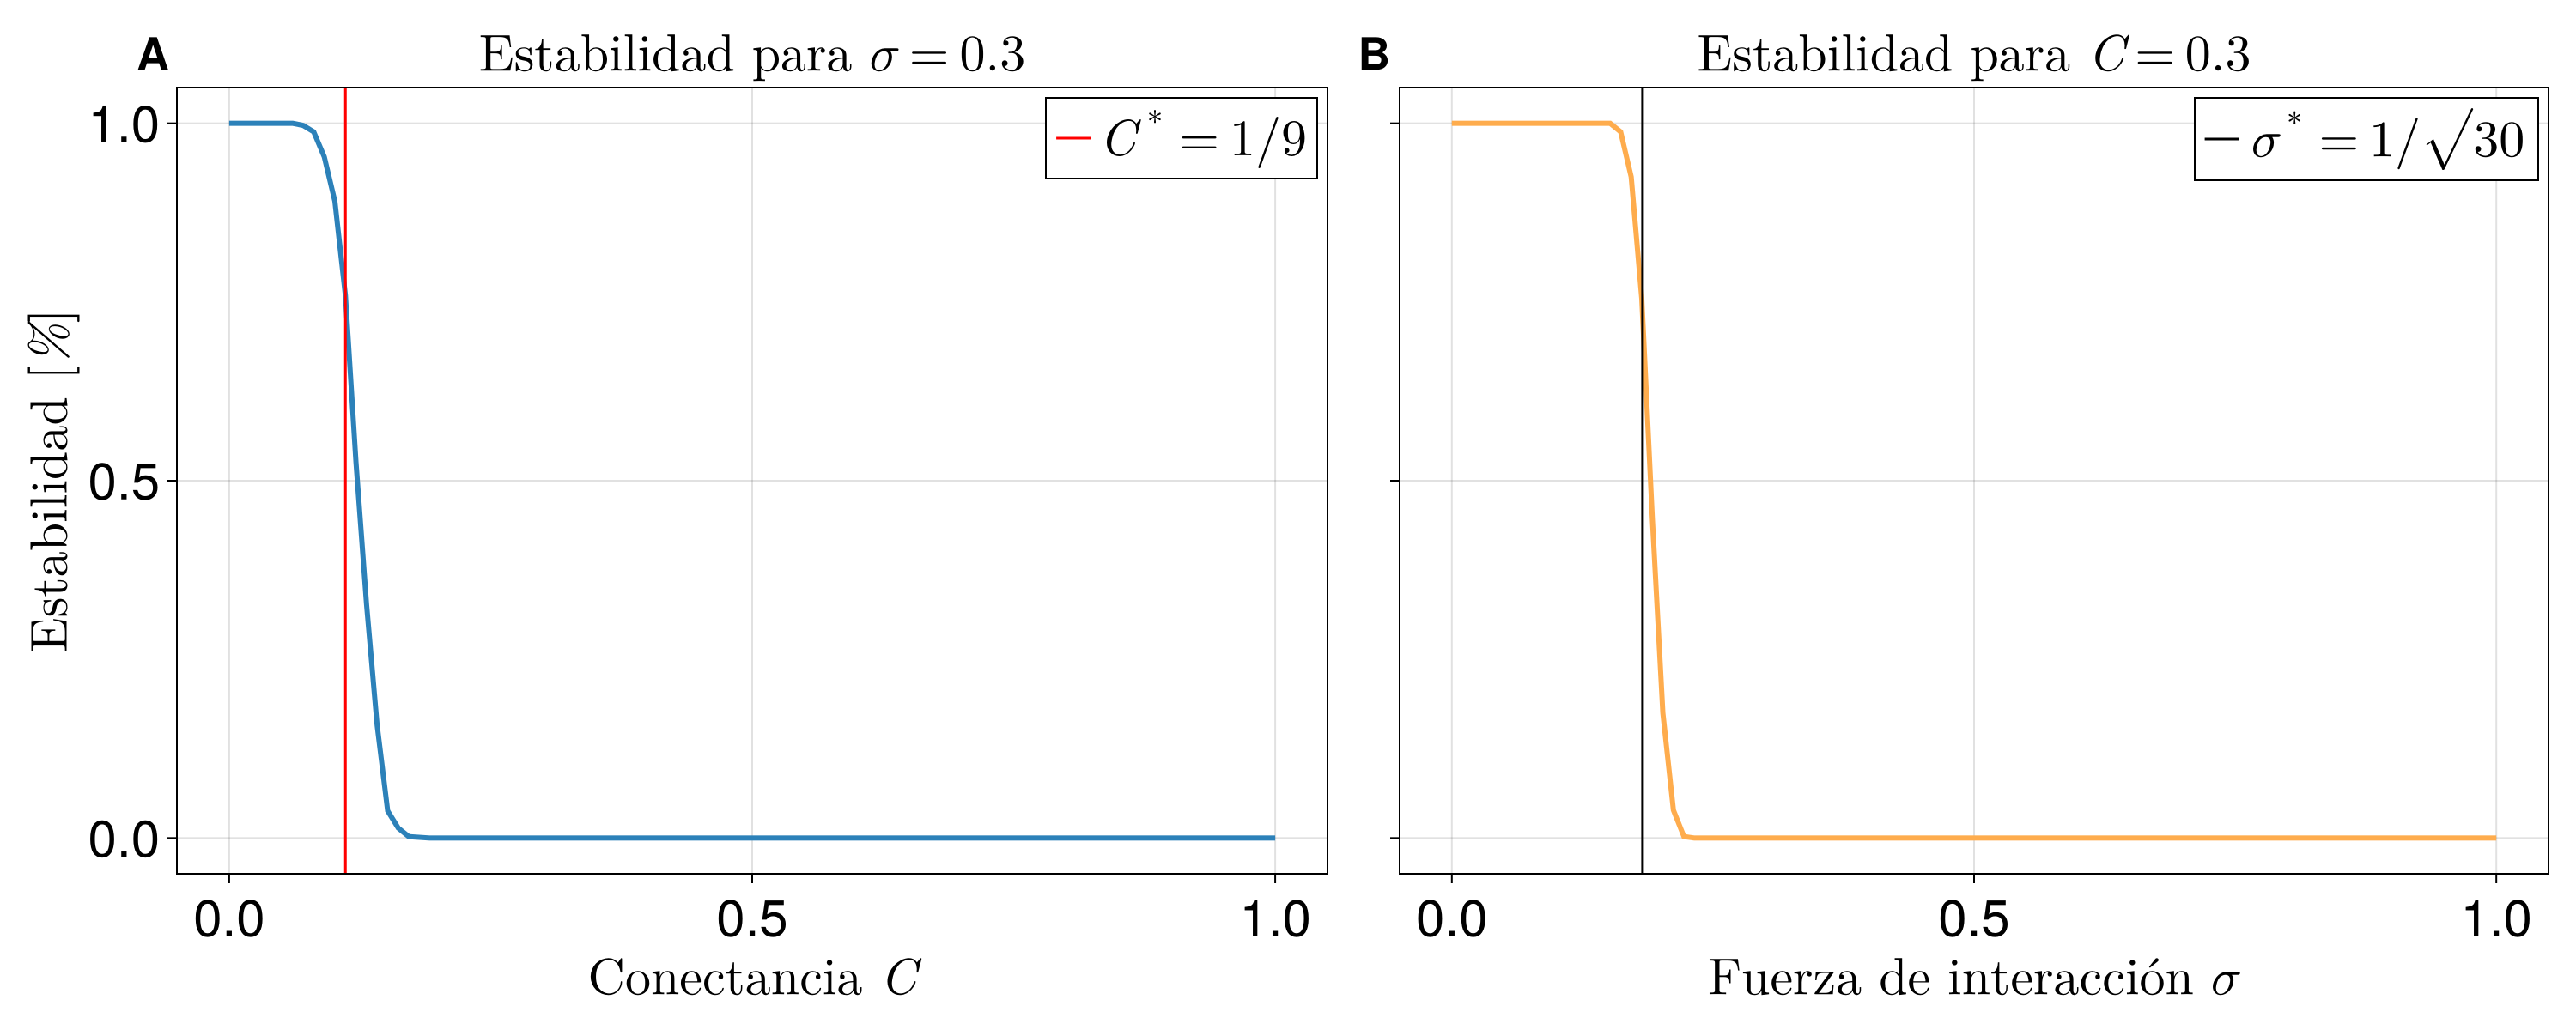
\includegraphics[scale=0.16]{../Imagenes/TransicionesdeMay}
	\caption{Transiciones de estabilidad con sistemas de May. (\textbf{A}) Para la conectancia variable y fijando $\sigma=0.3$. (\textbf{B}) Para la fuerza de interacción promedio variable y fijando $C=0.3$.}
	\label{fig:TransicionesdeMay}
\end{figure}

De aquí se puede observar que los puntos de transición toman el siguiente orden $C^*<\sigma^*$, es decir, que las transiciones en función $C$ ocurren en general primero que las transiciones en función de $\sigma$ lo cual comprueba el ejemplo dado por la Figura (\ref{fig:TransicionesdeMay}). En consecuencia, el régimen de estabilidad en función de $C$ es más corto que en función de $\sigma$. Derivado de este breve análisis, May establece una última conclusión: un sistema será estable si existen pocas conexiones en la red y que las que existen tengan una fuerte interacción. En caso contrario, una red bien conectada podrá ser estable únicamente con interacciones débiles.
\newpage
\section{Planteamiento del problema}
%CHECKPOINT 2abril2025
Partiendo del hecho de que May ha llegado a sus conclusiones considerando \textit{a priori} sistemas lineales sin haber pasado necesariamente por el proceso de linealización, la misión de esta tesis es mostrar al lector una forma de construir estos sistemas no lineales, linealizarlos y llegar a un semejante de las matrices de May. Para ello se planea trabajar con el sistema de Lotka-Volterra generalizado \cite{may2007theoretical}
$$\frac{dx_i}{dt}=r_ix_i\left(1-\frac{\sum_{j=1}^N \alpha_{ij}x_j}{K_i}\right)$$
Las $r_i$ y $K_i$ son las tasas de crecimiento y capacidades de carga provenientes de la ecuación logística (\ref{eqn:EqLogistica}), mientras que las $\alpha_{ij}$ son las interacciones de las especies $x_j$ con la especie $x_i$. Tal y como se mencionó en la introducción, este sistema puede ser más que de competencia, se le pueden agregar otras interacciones que enriquecen la dinámica resultante. Se considera construir para $N\gg 1$, por lo que es prácticamente imposible de resolver analíticamente, para ello se ocuparan algoritmos computacionales e integración numérica con intenciones de modelar y resolver. \\
\\
Se comenzará modelando las interacciones $\alpha_{ij}$ del sistema; se va a construir una matriz a la que se denominará como \textit{matriz de incidencias}, en ella se guardarán únicamente los coeficientes de interacción del sistema. Esta matriz es la representación de una red \cite{newman2018networks}, donde cada nodo representa una especie y los enlaces tienen asociado un peso, los $\alpha_{ij}$ respectivamente. Una de las ventajas de esta matriz es que tiene la opción de tener diversas topologías de red, para este trabajo únicamente se ha considerado el modelo de \textit{red aleatoria} de Erdös–Rényi \cite{posfai2016network}. En el siguiente capítulo se hablará con más detalle de su construcción, por ahora solo queda mencionar que esta matriz también es gobernada por 3 parámetros: $p$, $\sigma$ y $N$, el primero representando la probabilidad de relación entre especies, el segundo la magnitud de sus interacciones y el tercero el tamaño del sistema. \\
\\
Habiendo introducido la propuesta para las interacciones de las ecuaciones de Lotka-Volterra generalizado y teniendo a disposición las herramientas computacionales para resolverlo, ¿cuál sería la conjetura a abordar? Se quiere mostrar que existe una transición de fase de un estado ordenado (estable) a uno desordenado (inestable). Para llegar a ese punto se debe comenzar por hallar los puntos fijos donde se evaluará la estabilidad. Esta no es una tarea trivial debido a la cantidad de puntos fijos que pueden existir, más aún, encontrar si existe alguno que resulte estable. Al efectuar la integración numérica se pueden hallar pistas sobre los puntos fijos: si la serie de tiempo diverge entonces es más que evidente que el sistema es inestable, en caso contrario entonces este valor al que se estabiliza puede ser considerado un atractor del sistema.
\newpage
Lo siguiente será linealizar el sistema por medio de su matriz Jacobiana evaluada en el punto fijo (una vez que se haya determinado) y con ello confirmar su estabilidad en términos de sus valores propios. Posteriormente se explorará la distribución espectral de las matrices Jacobianas generadas realizando un análisis comparativo con respecto de la Ley Circular de May. Estas distribuciones son el parámetro de orden de las transiciones de fase, será cuestión de estudiar que condiciones inducen a diferentes escenarios en la parte real de los valores propios\footnote{Re$(\lambda(\mathcal{J}))<0$, Re$(\lambda(\mathcal{J}))=0$ y Re$(\lambda(\mathcal{J}))>0$.}. \\
\\
Finalmente se medirá la probabilidad de estabilidad de los sistemas en función de $p$, $\sigma$ y para diferentes tamaños $N$ de la matriz de incidencias, tal y como se mostró en la Figura (\ref{fig:TransicionesdeMay}). Esto permitirá conocer la fase ordenada (estable) y la fase desordenada (inestable) del sistema verificando si el parámetro crítico se acopla con la desigualdad (\ref{eqn:paramMay}) de May. Para cada parte de la conjetura se presentan las siguientes hipótesis:
\begin{itemize}
	\item[1.] La serie de tiempo de un sistema con cierta configuración $\sigma$, $p$ y $N$ favorable en donde no divergen sus cantidades, presenta un punto fijo atractor y se le asocia al último valor $N$-dimensional de la serie. %En este sentido, existe una vecindad alrededor del atractor para la que se asegura la estabilidad del sistema.
	\item[2.] Las matrices Jacobianas de los sistemas no-lineales presentan una diagonal heterogénea a diferencia de las matrices de May en donde se encuentran fijadas a $-d$.
	\item[3.] Los elementos de las diagonales fungen el papel de centros y radios ``locales'' de Leyes Circulares que encierran valores propios en el plano complejo de matrices Jacobianas del sistema.
	\item[4.] El parámetro crítico de transición de estabilidad en las simulaciones generadas se encuentra asociado a la desigualdad $\sigma\sqrt{Np}<d$, donde la $d$ es un valor significativo de la distribución de valores de la diagonal.
\end{itemize}
